\section{Hardwareentwicklung, Softwarebackend \\ und Benutzeroberfläche \textcolor{gray}{(Benedikt Simbürger)}}

\subsection{Hardware}

\subsubsection{Planung - Grundanforderungen}
Grundlegende Anforderungen zur planung der AFSS-Mechanik, sind die größe des Lifts an der HTL-Mössingerstraße, sowie möglichst einfache realisierung mit HTL-mitteln, möglichst wenig kompromisse in der Funktion oder zuverlässigkeit eingehen zu müssen.
Die Anforderung der Transportfähigkeit limitiert die Größe des Lagers auf 2.3 m Länge um im Lift transportiert werden zu können und auf 1.9 m höhe aufgrund der Türhöhe im Keller. Weiters müssen auch noch Rollen an den Rahmen angebracht werden, um das Lager überhaubt erst ohne großen mehraufwand bewegen zu können. Diese Extrahöhe limitiert den Rahmen weiter.
Nun soll dieser rund 2.25 m lange und 1.8 m hohen Raum optimal genutzt werden um eine möglichst große Lagerdichte sicherstellen zu können.
Um möglichst gute erweiterbarkeit, sowie eine Fertigung an der Schule zu ermöglichen, sollen für die mechanische Trägerkonstruktion sog. Item-Profile verwendert werden. 

\begin{wrapfigure}{r}{0.3\textwidth}
    \vspace{0mm}
    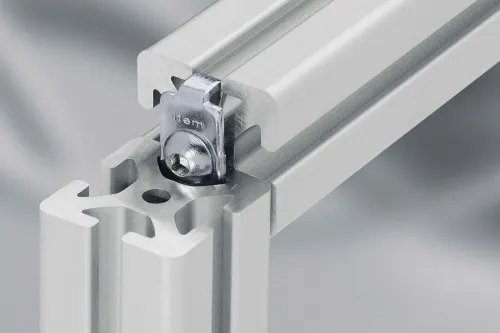
\includegraphics[width=0.3\textwidth]{Item-Standartverbindungssatz.png}
    \centering
    \caption{Item Profil mit Standartverbindungssatz, Quelle: \cite{Item_svs}}
\end{wrapfigure}
\paragraph{Item}\mbox{}\\
Das Item-Profilsystem, ist ein System welches Aluminium Extrusionen in verschiedenen Ausführungen, sowie viele Verbindungs-möglichkeiten zu sich selbst sowie andere mechanische Elemente bietet. Hierbei gibt es eine breite Auswahl an Profielen, von 20x20 mm bis 40x40 mm Querschnitt. Für alle Komponenten mit hoher mechanischer Beanspruchung werden 40x40-Extrusionen verbaut, da diese eine besonders hohe Biegefestigkeit aufweisen. Für Anwendungen mit geringerer Beanspruchung sowie aus Platz- und Gewichtsparmaßnahmen, werden 20x20-Extrusionen Verbaut. 
Zur Verbindung zu anderen Bauelementen gibt es die Möglichkeit sog. Nutenstene mit verschiedenen Gewinden in die Nut einzulegen und dort Platten o. ä. anzuschrauben. Um Item-Profile untereinander zu verbinden, werden Standartverbindungssätze verwendet. \\

Die Anwendung im AFSS erfordert weiters recht lange Verfahrwege. Um dies kostengünstig umsetzen zu können, werden V-Slot Profile verwendet


\begin{wrapfigure}{R}{0.3\textwidth}
    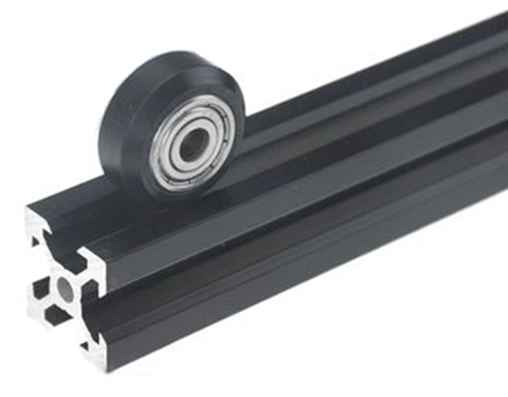
\includegraphics[width=0.3\textwidth]{V-Wheel.jpg}
    \centering
    \caption{V-Slot-Profil mit V-Wheel, Quelle: \cite{v_slot_wheel}}
\end{wrapfigure}
\paragraph{V-Slot}\mbox{}\\
Auch V-Slot-Profile sind Aluminium Extrusionen. Diese können grundsätzlich auch ähnlich wie Item-Profile, mit Nutensteinen ect. verwendet werden, sind aber zusätzlich darauf ausgelegt, dass ein V-Wheel in einer Narbe des Profils rollen kann. Dies Profile sind in einer C-Profil-Form erhältlich. Diese sind für die langen Verfahrwege optimal, da diese einerseits auch breiter und mehr V-Wheels verwendet werden, sowie einen sehr großen Widerstandsmoment aufweißen. 


\subsubsection{Vorgehensweise}
Aufgrund der besoderen und sehr Komplexen anforderungen dieser Mechanik, erfolgt die Entwicklung in mehreren Iterationen. Nach Auslegung der Grundparameter wird eine Grundkonstruktion erstellt, um mögliche Lösungsansätze für die jeweiligen Komponenten zu skizzieren. Durch diese Grobe Planung, können viele Konzepte ohne großen Zeitaufwand iteriert werden und auch mögliche missverständnisse o. ä. frühzeitig aufgeklärt und überarbeitet werden. \\
Um bestimmte elemente der Mechanik einzeln zu testen, werden auch mehrere Prototypen gebaut und die gewonnenen Erkentnisse in die finale Konstruktion miteingebunden. \\

\begin{figure}[H]
    \centering
    \begin{subfigure}{.3\textwidth}
        \centering
        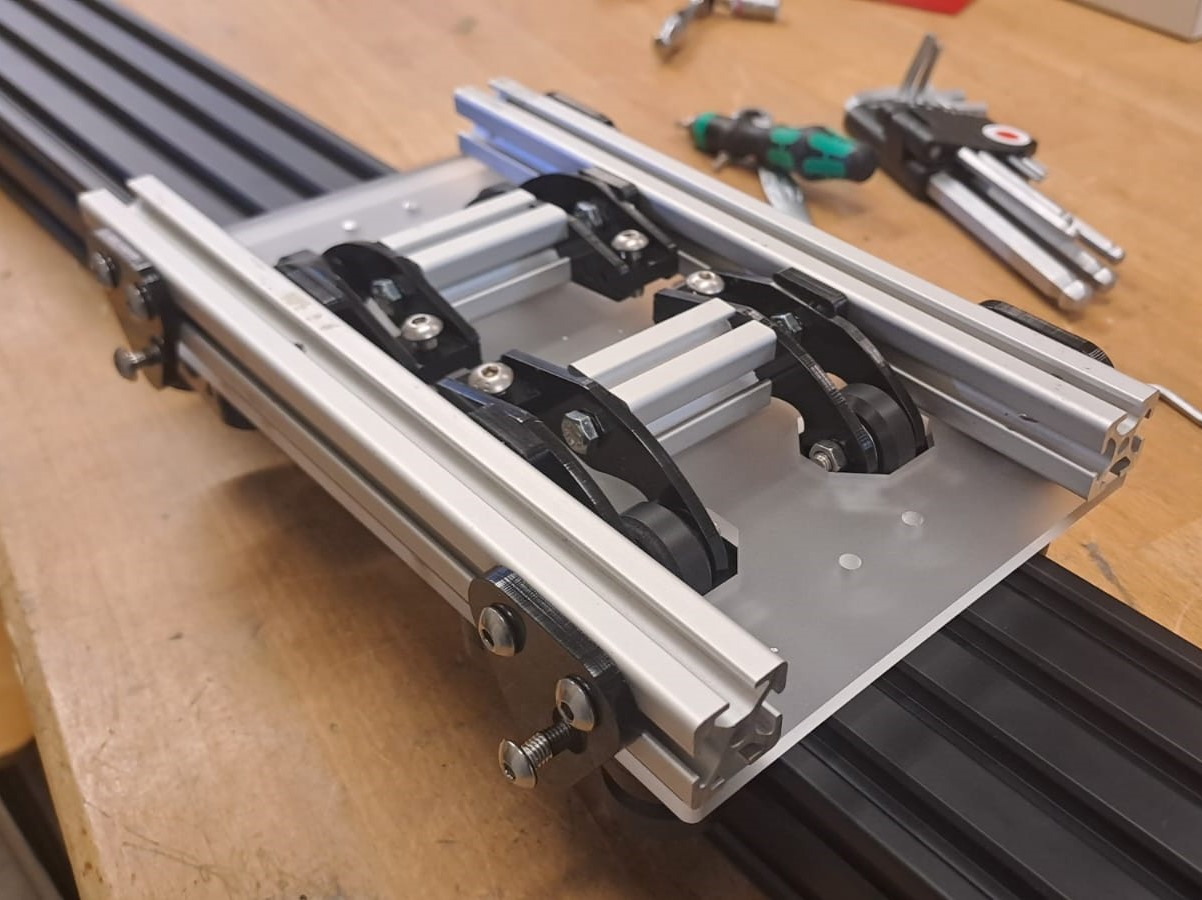
\includegraphics[width=0.9\textwidth]{pt_x.jpg}
        \caption{X-Achse}
        \label{pts:plt_x}
    \end{subfigure}%
    \begin{subfigure}{.3\textwidth}
        \centering
        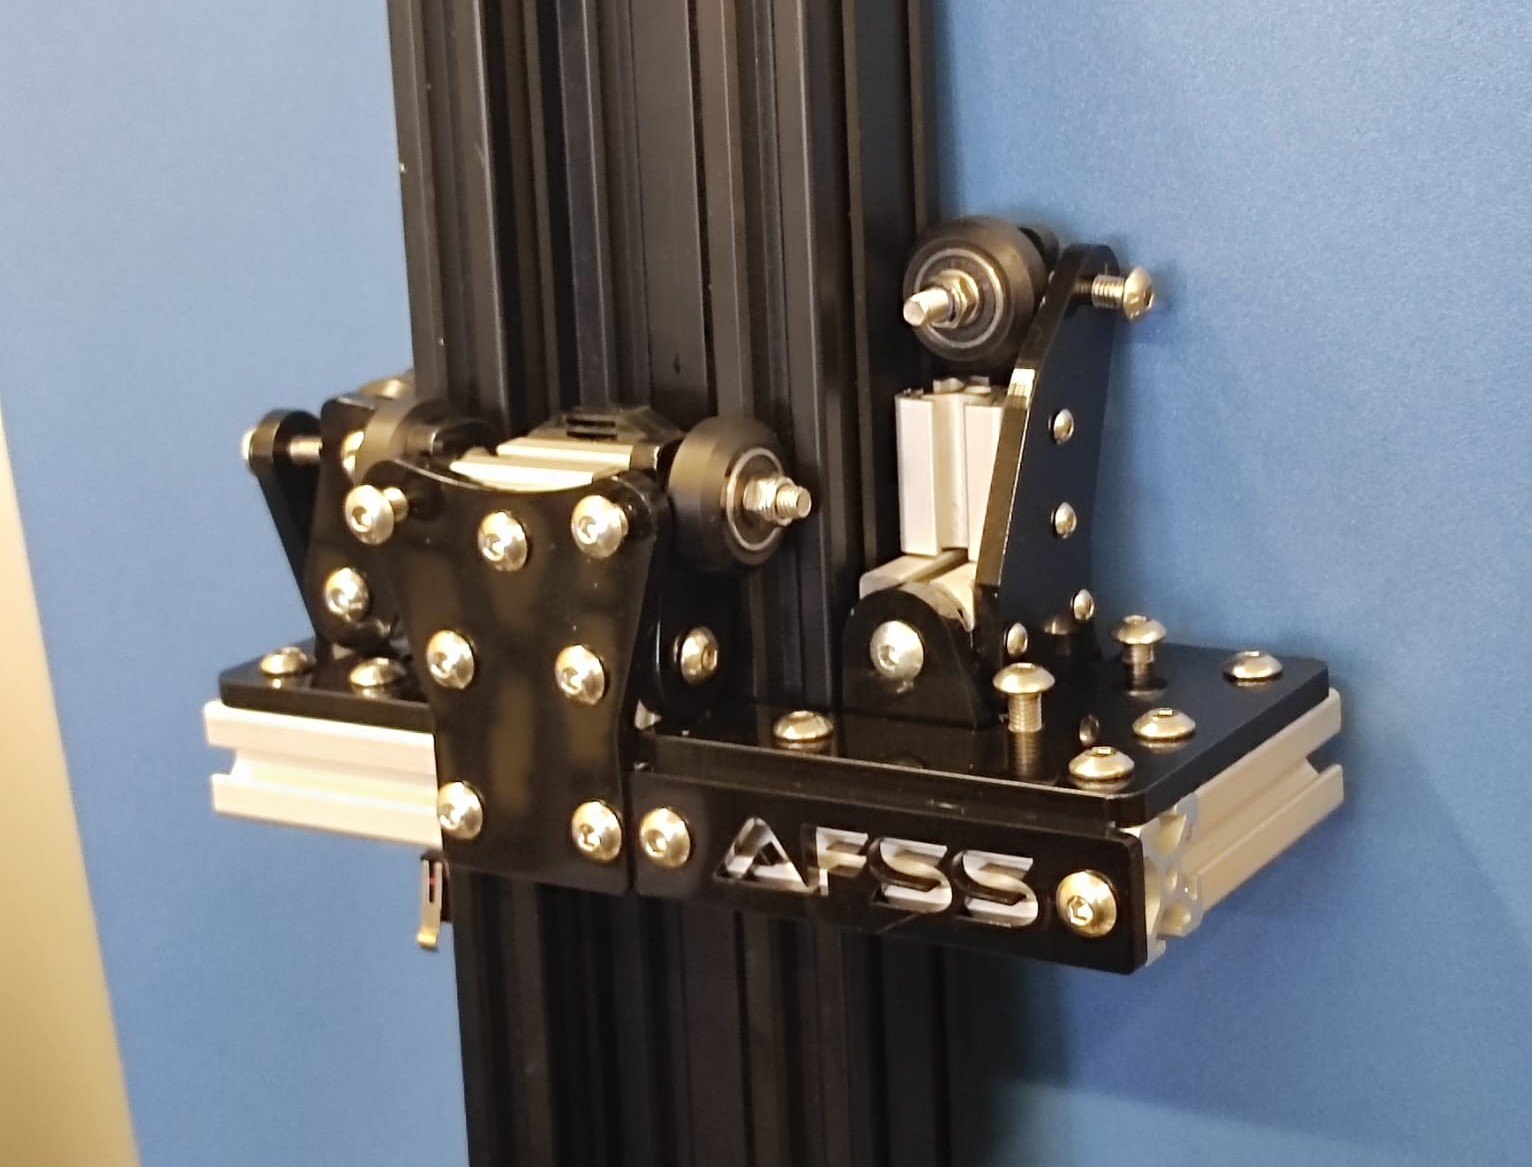
\includegraphics[width=0.9\textwidth]{pt_y.jpg}
        \caption{Y-Achse}
        \label{pts:plt_y}
    \end{subfigure}%
    \begin{subfigure}{.3\textwidth}
        \centering
        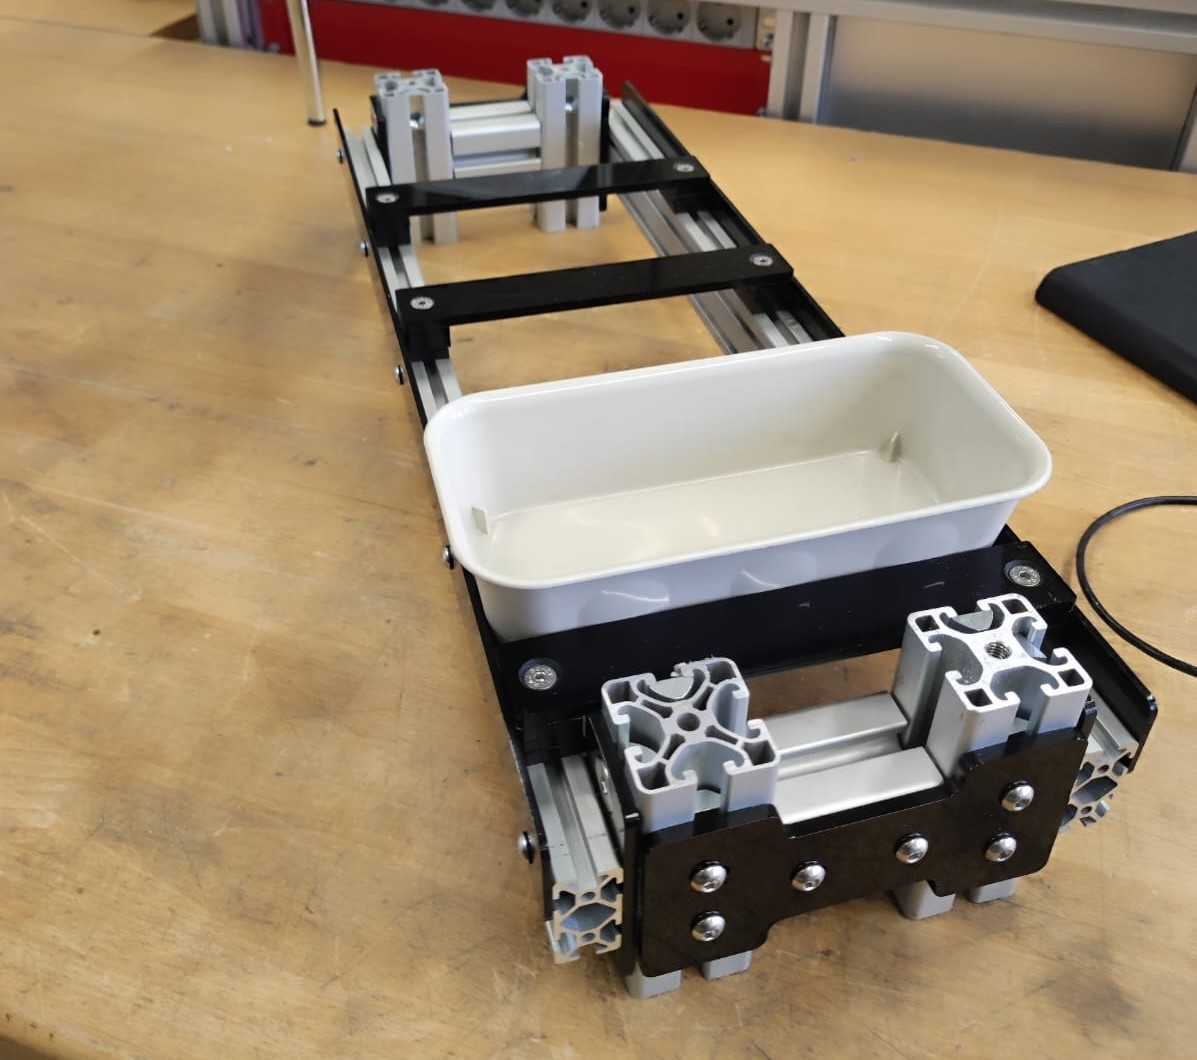
\includegraphics[width=0.9\textwidth]{pt_lg.jpg}
        \caption{Lagerregal}
        \label{pts:plt_ls}
    \end{subfigure}
    \caption{Prototypen}
    \label{pts}
\end{figure}

\subsubsection{Fusion360}

\subsubsection{Rahmen}

Der Rahmen des AFSS bezeichnet jene Struktur, welche als äußerstes Gehäuse, sowie grundlegende mechanische Stabilität bietet. Es ist geplant, dass es die anforderungen von Maximalhöhe und -länge optimal ausnutzt sowie breite minimal hält. \\
Umgesetzt wird dies mit einem Gerüst aus 40x40-Aluminium Extrusionen. Dieses hat weiters oben udn unten noch zwei Längsstreben, die dazu dienen, eine möglichst platzsparende aufhängung, der X-Achsen V-Slot-Profile, zu realsisieren. Auf einer Seite wird weiters eine Aussparung eingeplatn, um genug Freiraum übrig zu lassen, damit der Querförederer die Boxen reibungslos auf das Förderband bringen kann.\\
Weiters muss noch eingeplant werder, dass noch Rollen zum Transport angebracht werden müssen. Dadurch, dass diese auswirkungen auf die Maximalhöhe haben, muss dass in die Auslegung der Y-Achse einfließen, um Bewegung durch Türen zu ermöglichen.

\subsubsection{X-Achse}
Die X-Achse des AFSS ist das Mechanische Herzstück. Sie ist jene Achse, welche sich horizontal beweget. Sie hat einen langen Verfahrweg und hohen mechanische Anforderungen (sie muss ihr Eigengewicht und das Gewicht der YZ-Achse stützen). 
Grundelement der X-Achse sind V-Slot C-Profile, welche oben und unten aufgehängt werden. Diese sind in 1.5 m länge erhältlich, deshalb wird die ganze Achse darauf ausgelegt, 2 Stück also 3 m Schiene zu verwenden. Diese sind weiters mit 6 Nivelierungsschrauben pro V-Profil ausgestattet, um diese möglichst Parallel zueinander sowie in Waage zu positionieren.

\paragraph{Schlittenauslegung}\mbox{}\\
Auf der X-Achse verläuft der X-Schlitten, dieser hat die Aufgabe die Y-Achse zu positionieren. Um dies zu bewerkstellingen, muss dieser alle nötigen Motoren und Sensoren beinhalten. Weiters muss er einen Angriffspunkt bieten, um diesen zu bewegen. Ausserdem soll der Schlitten horizontal und vertikal möglichst kompakt sein, um einen möglichst großen Verfahrweg in X- als auch Y- Richtung zu ermöglichen.
Um eine möglichst Reibungsarme bewegung bewerkstelligen zu können, werden

\paragraph{Antrieb}\mbox{}\\
Angetrieben wird die X-Achse mit zwei Schrittmotoren, welche jeweils an einer Schiene (oben und unten) angebracht werden. Diese treiben mithilfe eines Zahnriemen die zwei X-Schlitten an. Als Zahnriemen wurde aufgrund der hohen Kraftübertragung, sowie großer Länge auf ein AT5-Zahnprofil mit 16 mm Riemenbreite der Firma Mähdler gesetzt. Dieser wird vom Motor über eine Entsprechende Zahnscheibe angetrieben, und am Shuttle befestigt. Als Schrittmotor wird aus einfachheitsgründen das selbe Modell wie bei der Y-Achse verwendet. Diese erzeigen auch genügend Moment um die X-Achse anzutreiben.

\paragraph{Riemenspannung X-Achse} \mbox{}\\
Da der Riemen für eine zuverlässige Kraftübertragung bei so langen Verfahrwegen eine relativ große Vorspannkraft benötigt wird, ist das Zahnriemenklemmelement auf der X-Achse auch dementsprechend auszuführen. Um den Zahnriemen zu greifen, muss ein Negativ in Aluminium gefräßt werden, in dieses der Zahnriemen dann auf beiden Seiten des Schlittens geklemmt wird. Die Aufhängung der einen Seite ist einfach mit den Item-Profilen verschraubt, lässt aber noch etwas platz, um den Riemen mit der Hand vorzuspannen. Auf der anderen Seite ist das Klembrett über zwei Gewindestangen mit dem restlichen Shuttle verbunden. Diese können festgezogen werden, um die nötigen Vorspannkräfte zu erzeugen. Ausserdem ist diese Spannvorrichtung in einem Formfaktor ausgeführt, welcher es erlaubt, dierekt darüber die Motoren der Y-Achse anzubringen. 

\paragraph{Achsenführung} \mbox{}\\
Die Fürung der Achse im V-Slot-Profil wird mit V-Wheels durchgeführt. Sechs V-Wheels werden von oben auf das C-Profil gedrückt. Jedes Rad wird einzeln aufgehangen. Weiters ist überall eine Schraube mit welcher das Rad weiter in die Führung hienein gedrückt werden kann, sowie ein bis zwei Klemmpunkte, um bei Betrieb die Last von der Spannschraube nehmen zu können. \textbf{Durch den Geringen Platz im Schlitten ist es durchaus ein Triumpf, dass alls diese Mechanik, neben der Spannelemente und Motoren in einem so kleinen Shuttel platz finden.} Auf der Seite des Schlittens werden noch weitere V-Wheels angebracht, welche die Spurführung übernehmen.
Im oberen Schlitten werden nur diese Fuhrungsräder verbaut, da es nicht möglich und nötig ist, vertikale Kräfte zu unterstützen.

\paragraph{Kabelführung} \mbox{}\\
Um Sensoren und Aktoren der Y- und Z-Achse zu unterstützen, müss dementsprechende Leitungen auf das X-Shuttel verlegt werden. Die wird mithilfe einer Kabelschleppkette der Firma Igus umgesetzt. Diese wird pralell zum unteren C-Profil verlegt und unter berücksichtigung der Biegeradien am X-Shuttel befestigt. Bei dieser ist darauf zu achten, dass sie alle benötigten Leitungen, sowie genügent Freiraum für die Biegung einhält. Weiters müssen Signal- und Aktorstromkreise durch trennstege voneinander getrennt werden.\\
Um die weiteren Geräte am  AFSS zu versorgen, müssen zusätzlich noch Kabelkanäle am Rahmen angebracht werden. 

\paragraph{Sensoren}\mbox{}\\
Die Sensorik ist bei jeder Achse ähnlich aufgebaut. Immer zwei Endschalter und ein Referenzierschalter. Bei der X-Achse werden als Endschalter mechanische Rolltaster verwendet. Diese werden neben den V-Slot-Profilen befestigt und von einem, vom Schlitten abstrehenden Arm ausgelöst. 


\subsubsection{Y-Achse}
Als Y-Achse wird jene Achse bezeichnet, die ihre Bewegung vertikal durchführt. Sie hat die Aufgabe, die Z-Achse bzw. das YZ-Shuttel auf Position zu bringen. Wichtig hierbei ist jedoch, dass die Y-Achse die Aufgabe des aufheben der Box übernimmt.

\paragraph{Antriebsauslegung}\mbox{}\\
Dadurch, dass die Y-Achse sowohl YZ-Shuttle als auch die Boxen aufheben muss, muss der Antrieb dementsprechend dimensioniert werden. Als Formfaktor sol ein Nema23-Schrittmotor verwendet werden. Diese sind weit verbreitet und zu Servomotoren verhältnissmäßig kostengünstig. Als grundformfaktor wird ein 2 Nm Motor gewählt, nun soll überprüft werden, ob dieser die Last der YZ-Achse auch antreiben kann.

\vspace{5mm}
\noindent\begin{minipage}{\textwidth}
\begin{minipage}[t]{0.5\textwidth}
    \begin{equation*}
        F = \frac{M}{\frac{d}{2} \cdot 1000} \cdot n
    \end{equation*}
    \begin{equation*}
        F = \frac{2 \unit{Nm}}{\frac{30 \unit{mm}}{2} \cdot 1000} \cdot 2 = 266 \unit{N}
    \end{equation*}
\end{minipage}%
\begin{minipage}[t]{0.4\textwidth}
    \vspace*{-5mm}
    \begin{align*}
        &F: \text{Antriebskraft der Y-Achse} & &\left[N\right]\\
        &M: \text{Drehmoment eines Motors} & &\left[Nm\right]\\
        &d: \text{Durchmesser der Antriebszahnscheibe} & &\left[mm\right]\\
        &n: \text{Anzahl der Antriebe} & &
    \end{align*}
\end{minipage}
\end{minipage}

\vspace{5mm}

Bei Konstruktion einer früheren Version des YZ-Shuttels wurde erfasst, dass das Shuttel bis zu 13 kg Wiegen kann. Dies wird zwar in einer späteren Iteration des Designvorgangs noch verbessert, dient jedoch als richtwert der Antriebsauslegung. 13 kg erzeugen ohne berücksichtigung von Reibung knapp 130 N. Die Antriebskraft der Schrittmotoren reicht auf jeden fall aus. Doch diese Überdimensionierung ist unter dem Aspekt, dass die Antriebe über keine Bremse verfügen, also das gesamte Gewicht immer unterstützen müssen, durchaus sinnvoll.


\paragraph{Zahnriemen und Umlenkung}\mbox{}\\
Als Zahnriemen wird auch bei der Y-Achse auf eine AT5x16-Profil gesetzt. Doch hier gestaltet sich die Positionierung ebendieses nicht so simpel wie bei der X-Achse. Da der Zahnriemen beim YZ-Shuttle an einem bestimmten Punkt befestigt werden muss, muss er auch dort wieder Rückgeführt werden. Die Umlenkung des Zahnriemens gestaltet sich jedoch wesentlich anspruchsvoller als bei der X-Achse, da einerseits ain möglichst kompakter Formfaktor angestrebt werden muss, sowie andererseits eine aufhängungstechnisch sehr unvorteilhafte Positionierung vor dem V-Slot C-profil erforderlich ist. Aus diesem Grund wir eine konstrukiton aus Aluminium, welche sich selbst verhakt konstruiert. Sie muss Seitlich ann den Profilen verschraubt werden. Im forderen Überhang werden Aluminiumelemente eingehängt, welche die Aufhängung der Achse für die Umlenkung erlauben. 


\paragraph{Positionsbestimmung der Zahnriemenaufgängung}\mbox{}\\

Um die optimale Postiton der Zahnriemenaufhängung für die Y-Achse bestimmen zu können, wird überschlagsmäßig ein Massenschwerpunkt in Z-Richtung berechnet. Um die Konstrukiton beginnen zu können, werden hierfür ungefähre werte angenommen.

\noindent\begin{minipage}{\textwidth}
\begin{minipage}[t]{0.5\textwidth}
    \vspace{7mm}
    \begin{equation*}
        X_s = \frac{1}{M} \cdot \displaystyle\sum_{i = 0}^{n} z_i \cdot m_i
    \end{equation*}
\end{minipage}%
\begin{minipage}[t]{0.5\textwidth}
    \begin{align*}
        &Z_s: \text{Z-Koordinate des Massenschwerpunkts} & &\left[m\right]\\
        &M: \text{Gesamtmasse} & &\left[kg\right]\\
        &z_1: \text{Z-Koordinate der Teilmasse} & &\left[m\right] \\
        &m_1: \text{Masse der Teilmasse} & &\left[kg\right]
    \end{align*}
\end{minipage}
\end{minipage}

\vspace{5mm}

    \begin{table}[H]
        \centering
        \centering
            \begin{tabular}{c c c}
                Gegenstand & Masse in kg & Position in mm\\
                \hline
                Motor & 0.3 & 21 \\
                Z-Schiene & 1 & 150 \\
                Z-Gable & 0.3 & 180 
            \end{tabular}
        \caption{X-Achse unbeladen und eingefahren}
        \end{table}
    \begin{table}[h!]
            \centering
            \begin{tabular}{c c c}
                Gegenstand & Masse in kg & Position in mm\\ 
                \hline
                Motor & 0.3 & 21 \\
                Z-Schiene & 1 & 150 \\
                Z-Gabel & 1.3 & 380
            \end{tabular}
            \caption{X-Achse beim Ladevorgang}
        \end{table}
    \vspace{5mm}

    So werden zwei Schwerpunkte errechnet: ca. 130 mm im unbeladen und 250 mm während dem Ladevorgang. Da die Stabilität des Y-Schuttels während dem Ladevorgang wichtiger ist als während einer Leerfahrt wird das Y-Shuttle so positioniert, dass die Aufhängung des Zahnriemen bei rund 200 mm liegt. 
    

\paragraph{Shuttleführung}\mbox{}\\
Das YZ-Shuttel wird aus Stabilitätsgründen ebenfalls mit einem V-Slot C-Profil geführt. Dieses sind auf beiden Seiten jeweils oben und unten befestigt. Die Länge wird so gewählt, dass die Verwendung eines 1.5 m langen Profils perfekt ausreicht. Da dass YZ-Shuttel wesentlich weniger Kraft auf die Führung auswirkt können weniger Führungsräder verwendet werden. Die Hauptführungsräder werden so Positioniert,  dass sich ein Dreieck ergibt. Dieses dient dazu, dass sowohl beim Aufhängevorgang als auch beim Leerlauf immer eine Klemmung um die Führungsschiene entsteht. Hierbei sind jene V-Wheels, welche beim Aufhebevorgang belastet werden, doppelt ausgeführt. Wie schon bei der X-Achse sind auch hier wieder alle V-Wheel-abstände mit Schrauben einstellbar. Zusätzlich zur Hauptführung sind auch aussen jeweils noch zwei Führungsräder angebracht, um das Shuttel zusätzlich zu stabilisieren.

\paragraph{Sensoren}\mbox{}\\
Da die Endschalter der Y-Achse kapazitiv ausgeführt sind, muss auf dem Shuttel ein Metallisches Gegenstück angebracht sein. Diese stehen uben und unten über und lösen so vor Kolission aus. Um die Sensoren anzubinden muss auch ein ASi-Client auf dem X-Shuttel angebracht werden.

\subsubsection{Z-Achse}


\subsubsection{Fertigung}

\paragraph{Umlenkrollen}\mbox{}\\
Die Umlenkrollen sind jeweils am Ende der X- und Y-Achsen angebracht. Dadurch dass diese der gesamten Spannkraft ausgesetzt. Dies erfordert spezielle Anforderungen an die Aufhängen als auch an die Umlenkrolle selbst. Diese soll primär eine 180° Wende des Zahnriemens ermöglichen, sowie sekundär eine Führung für den Riemen bieten. 
Umgesetzt wird diese Anforderungen, durch Fertigung von vier Aluminium-Drehteilen in welche Kugellager eingepresst werden.

\begin{figure}[H]
    \centering
    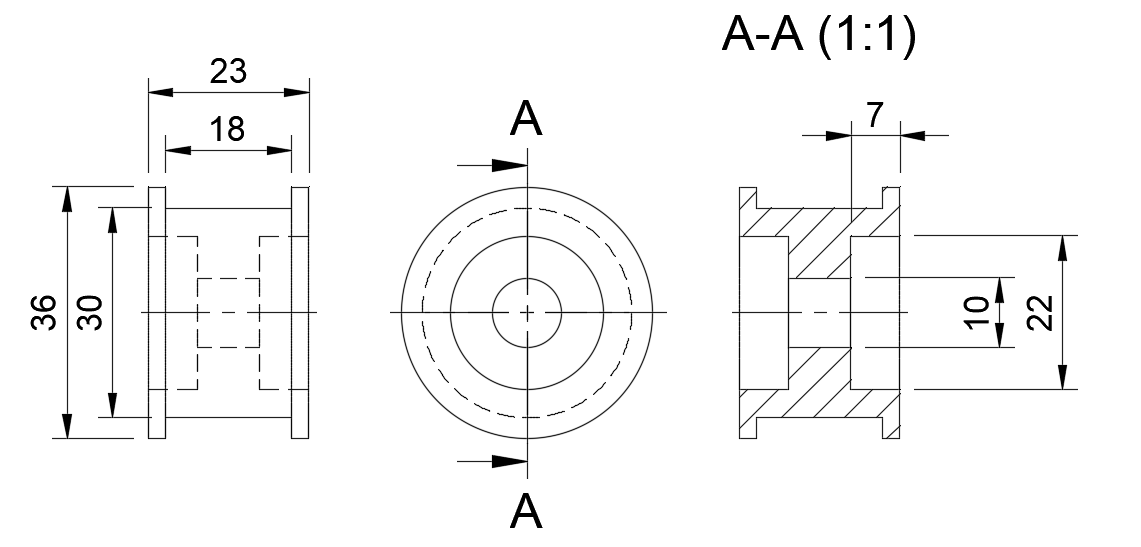
\includegraphics[width=0.8\textwidth]{AT5x16-Umlenkung.png}
    \caption{Bauteilzeichnung Umlenkrolle}
    \label{UmlenkrolleBTZ}
\end{figure}


Die Fertigung dieses Teils Lässt sich in folgende Teilschritte unterteilen:
\begin{itemize}
    \setlength\itemsep{-1mm} % Reduce space between items
    \item Zuerst die Frontfläche Plandrehen (900 U/min)
    \item Ungefär 30mm Länge auf das Aussenmaß von 36mm Plandrehen
    \item Mit 9.8mm Bohrer das mittlere Loch vorbohren (540 U/min)
    \item Mit 10mm Reibeisen und viel Öl das Loch auf eine genaue Passung bringen (260 U/min)
    \item Die Position relativ zum Backenfutter markieren, um beim Neu-Einspannen Rundlaufgenauigkeit zu gewährleisten
    \item Zylinder bei ca. 26 mm Abstechen (540 U/min)
    \item Umspannen und auf Maß Plandrehen (900 U/min)
    \item Die Aussparung für die Lager mit Eckdrehmeißel beginnen, jedoch nach innen hin nur 6.8 mm
    \item Bei ca. 17 mm Lochdurchmesser den tatsächlichen Durchmesser mit der Digitalanzeige vergleichen und gegebenenfalls korrigieren
    \item Bei 21.5 mm den Oberschlitten die restlichen 0.2 mm zustellen und die gesamte Tiefe Plandrehen
    \item Den Lochdurchmesser auf 21.95 erweitern und dann in kleinen Inkrementen zustellen, bis das Lager gerade so nicht passt, um einen Presssitz zu gewährleisten. Dies tritt bei Lagern mit 22 mm Außendurchmesser bei rund 22.04 mm ein.
    \item Da für die Einsparung der Riemenführungsfläche kein Angriffspunkt verfügbar ist, wurde als Halterung ein Dorn gedreht, auf welchen das Drehteil aufgeschraubt wird.
    \item Mit dem Abstechmeißel wird in 2 mm Inkrementen die Zahnriemenauflagefläche herausgedreht, bis auf 30.2 mm, sowie links und rechts den Rand 1 mm extra dick lassen. (540 U/min)
    \item Am Schluss wird der Rand auf Maß gedreht und die Tiefe fertiggedreht.
    \item Als letzten Schritt werden links und rechts die zwei Lager eingepresst.
\end{itemize}

    Durch die Verhältnissmäßig großen Toleranzen bei den Lageraussendurchmessern wird bei 2 der 8 Lagerpassungen zusätztlich Lagerkleber verwendet um eine Zuverlässige Passung zu gewährleisten.

    \begin{figure}[H]
        \centering
        \begin{subfigure}{.3\textwidth}
            \centering
            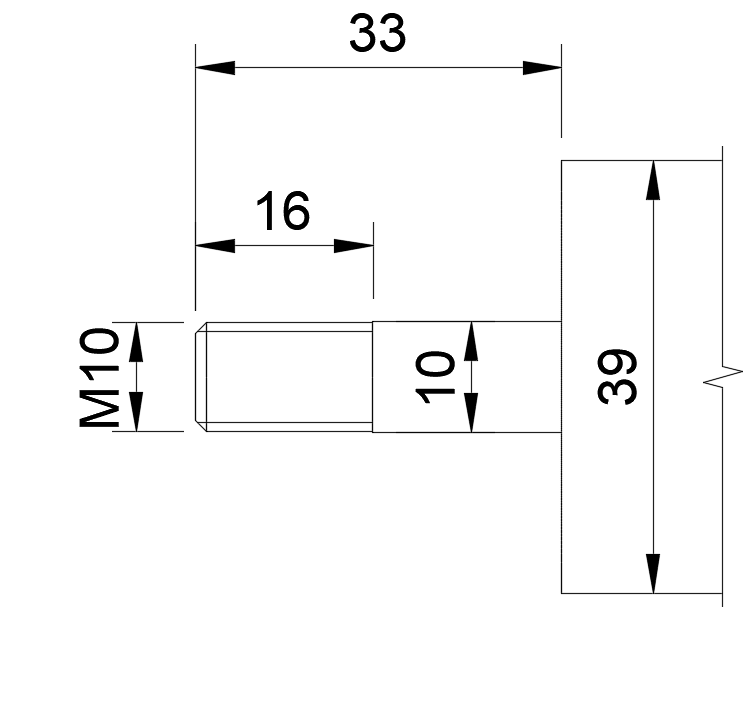
\includegraphics[width=0.9\textwidth]{AT5x16-Umlenkung-Dorn.png}
            \caption{Dorn}
            \label{ulr:dorn}
        \end{subfigure}%
        \begin{subfigure}{.3\textwidth}
            \centering
            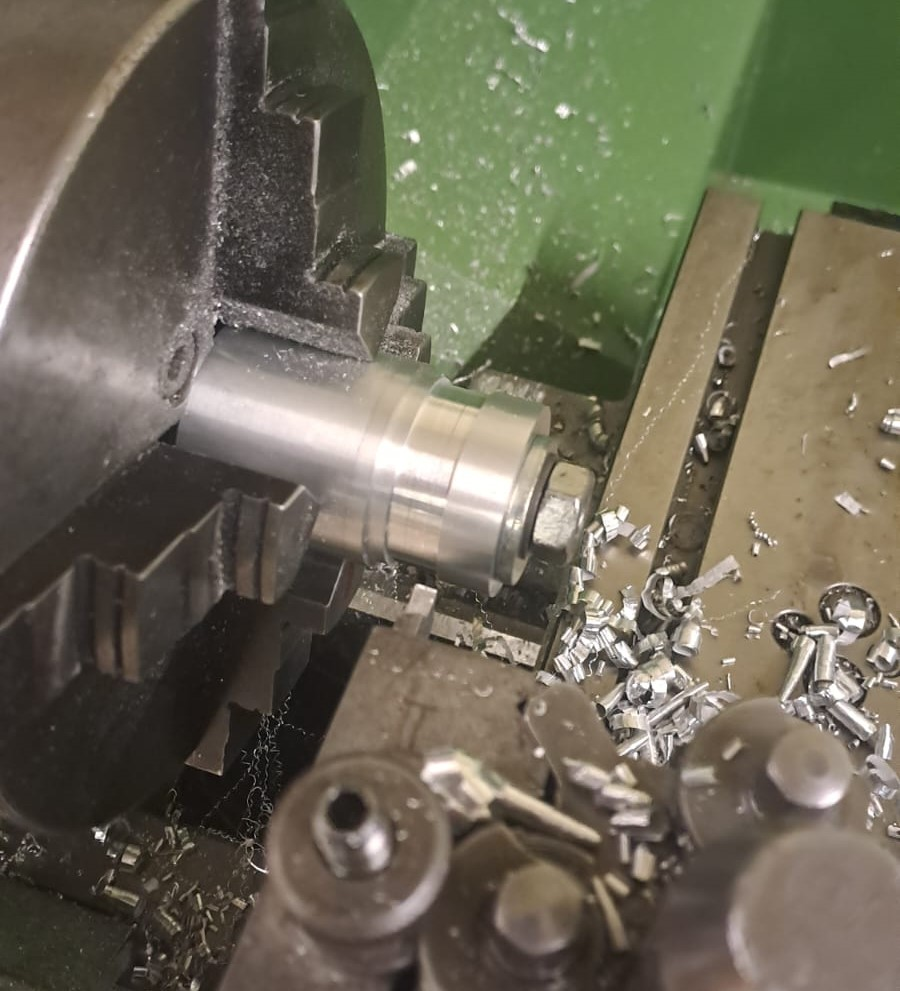
\includegraphics[width=0.9\textwidth]{ulr-fertigung.jpg}
            \caption{Fertigung}
            \label{ulr:f1}
        \end{subfigure}%
        \begin{subfigure}{.3\textwidth}
            \centering
            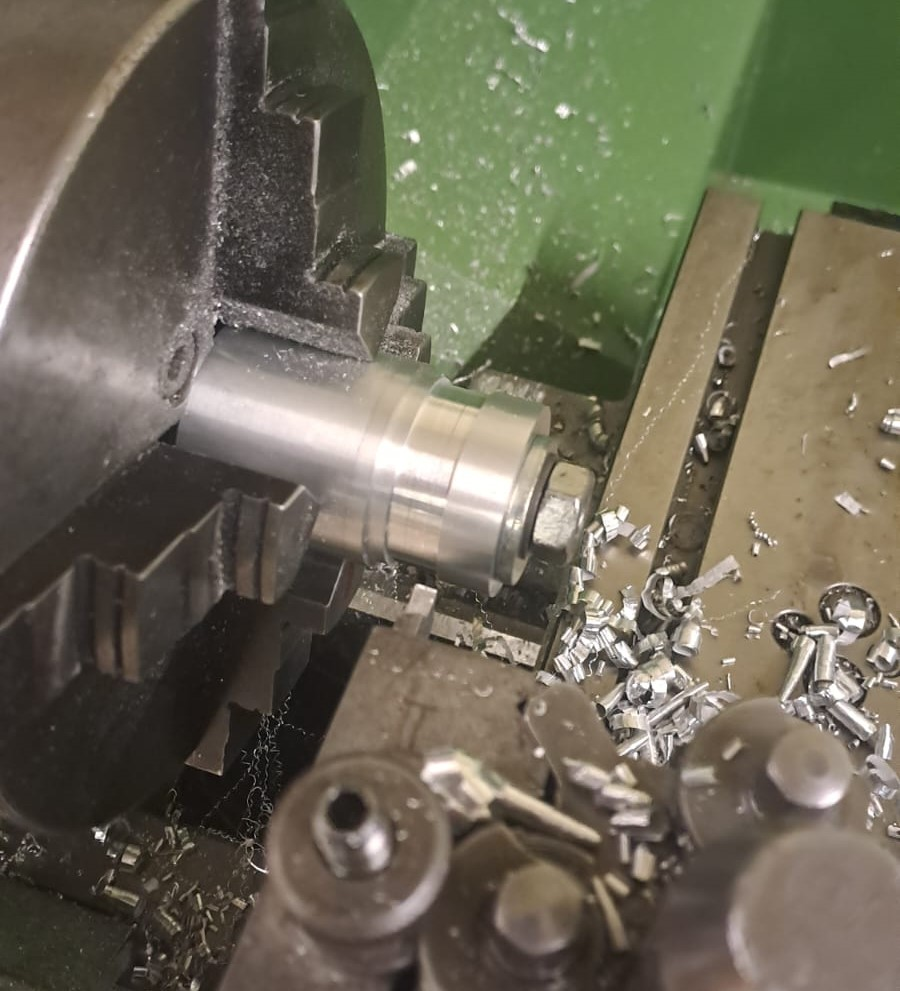
\includegraphics[width=0.9\textwidth]{ulr-fertigung.jpg}
            \caption{Fertig}
            \label{ulr:f2}
        \end{subfigure}
        \caption{Umsetzung der Umlenkrollen}
        \label{ulr}
    \end{figure}

\paragraph{Lasern}
\paragraph{Fräsen}

\subsubsection{Aufbau}

\newpage
\subsection{Software und Benutzeroberfläche}

\subsubsection{Grundlegendes}

Um dem Endnutzer die möglichkeit zu geben, das AFSS möglichst einfach zu bedienen, sowie die komplexen Logik zu Lagersteuerung auszuführen, bedarf es eines Servers (Backend) und einer graphischen Benutzeroberfläche (GUI oder Frontend). Diese müssen eine Vielzahl an Verschiedenen Funktionen beinhalten.

\subsubsection{Aufbau}
\begin{figure}[h]
    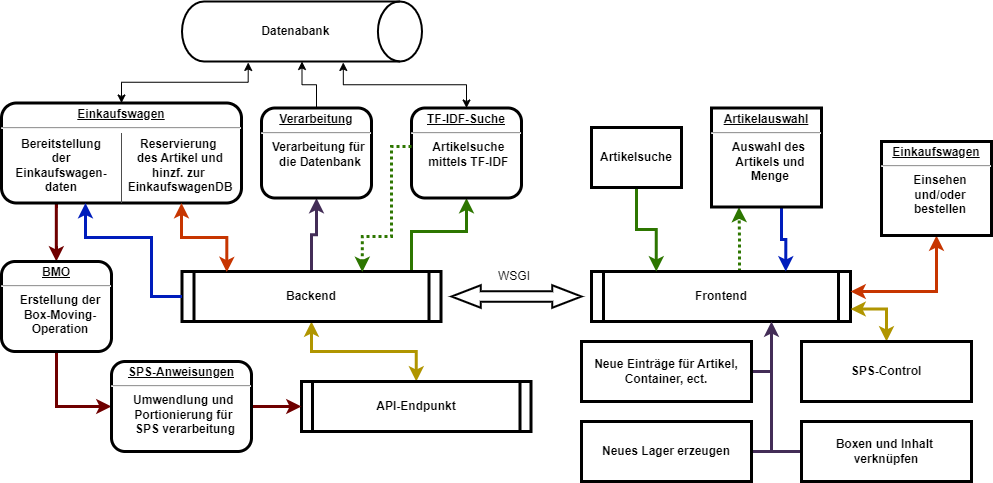
\includegraphics[width=\textwidth]{Software Howl.drawio.png}
    \caption{Gesamtüberblick des Servers}
\end{figure}

Um diesen Anforderungen gerecht zu werden, muss eine Lösung mit sehr hohem grad an Freiheit in der Logik sowie UI gestaltung gewählt werden. Weiters muss es möglich sein, dass zukünftige Schülerinnen und Schüler diesen instandhalten und erweitern. Aus diesen Gründen, sowie den bereits vorhandenen Kentnissen, wird die Programmiersprache 'Python' als Grundlage des Servers verwendet.

\paragraph{Python}\mbox{}\\
Python ist eine vielseitige und hochentwickelte Programmiersprache, die für ihre Einfachheit und Lesbarkeit bekannt ist und sich sowohl für Anfänger als auch für Fortgeschrittene eignet. Sie unterstützt mehrere Programmierphilosophien, darunter objektorientierte und funktionale Programmierung, und wird in Bereichen wie Webentwicklung, Datenanalyse, künstliche Intelligenz und wissenschaftlichem Rechnen häufig eingesetzt. \cite{python_wp}

\paragraph{Flask}\mbox{}\\
Flask ist ein leichtgewichtiges Web-Framework für Python, das durch seine Einfachheit und Flexibilität hervorsticht und sich ideal für kleinere Anwendungen oder Prototypen eignet. Es folgt einem minimalistischen Ansatz, bietet aber Erweiterungsmöglichkeiten, um komplexere Projekte zu realisieren. \cite{flask_wp}

\subsubsection{Benutzeroberfläche}

Um die Benutzeroberfläche zu realisieren muss eine Weboberflche erstellt werden. Auf dieser werden alle Inhalte angezeigt die für die Benutzung nötig sind. Sie wird vom Server zu verfügung gestellt, sobalt dieser eine http-Anfrage erhält. Um diese mit eigenen Inhalten und Funktionen zu befüllen, muss dies mit HTML geschehen.

\paragraph{HTML}\mbox{}\\

HTML (HyperText Markup Language) ist die Standard-Auszeichnungssprache zur Strukturierung und Darstellung von Inhalten im Web. Sie definiert die grundlegende Struktur einer Webseite mit Elementen wie Überschriften, Absätzen, Links, Bildern und Formularen. \cite{html_wp}

Dadurch, dass sich viele Elemente des UI wiederholen, wie z.B. Navigationsleiste, bietet Falsk die Möglichkeit sog. 'Templates' zu verwenden. Diese können einmal definiert werden und dann an mehreren teilen der Webseite verwendet werden.
Um elemente wie Formularflöchen oder Datenanzeige, einfach mit den benötigten Daten anzuzeigen, gibt die möglichkeit Macros zu erstellen, welche von Flask mit den bestimmten Daten vorgerendert und in das restliche HTML eingefügt werden.
Um HTML, welches grundsätzlich ohne Formatierung auskommt, zu stylen, muss CSS verwendet werden. 

\paragraph{CSS}\mbox{}\\
CSS (Cascading Style Sheets) ist eine Stylesheet-Sprache, die verwendet wird, um das Design und Layout von Webseiten zu gestalten. Sie ermöglicht die Trennung von Inhalt und Darstellung, indem sie Farben, Schriftarten, Abstände und andere visuelle Aspekte definiert.

Da auch Logik in der Webseite verbaut werden muss, muss zusätzlich auch Javascript verwendet werden, da HTML und CSS alleine, noch nicht gut genug mit dem Server Kommunizieren können.

\paragraph{JavaScript}\mbox{}\\
JavaScript (JS) ist eine vielseitige Programmiersprache, die hauptsächlich verwendet wird, um interaktive und dynamische Elemente auf Webseiten zu erstellen. Sie läuft direkt im Browser und ermöglicht Funktionen wie Animationen, Formularvalidierungen und die Kommunikation mit Servern in Echtzeit.

Praktisch geschieht diese Kommunkation immer mithilfe diese Programmblocks

\begin{lstlisting}[language=JavaScript]
    function sendData(data, callback) {
        var xhr = new XMLHttpRequest();
        var url = "{{url_for('main.add_stock')}}"; //Flask markup, um die richtige url zu erreichen, dies wird vor ausgabe auf der Webseite noch eingesetzt

        xhr.open("POST", url, true);
        xhr.setRequestHeader("Content-Type", "application/json");

        xhr.onreadystatechange = function () {
            if (xhr.readyState === 4 && xhr.status === 200) {
                callback(xhr.responseText)  //die funktion wir aufgerufen
            }
        };
        var jsonData = JSON.stringify(data);
        xhr.send(jsonData);
    }
\end{lstlisting}

Dieser ermöglicht die Übergabe von Daten im JSON format, und einer Funktion, die die zurückgeschickten Daten verarbeitet. In der Praxis wird dieser so aufgerufen:

\begin{lstlisting}[language=JavaScript]
function add_to_db(){
    sendData({"add_stock": {"barcode": barcode, "quantity": quant, "article": article}}, 
    set_gen_stock)
}

function set_gen_stock(req){
    document.getElementById("generated").innerHTML = req
}\end{lstlisting}

Wie im Quellcode ersichtlich, werden Daten aus der Webseite ausgelesen, in JSON konvertiert. Danach werden diese Daten zusammen mit einer Funktion, an 'send\_Data'. Wie bereits erwähnt, gibt der Webserver dann Daten zurück. In diesm Fall, werden dann Datten aus der DB vorvormattiert. Diese werden dann in der zuvor übergebenen Funktion, in der Webseite eingefügt.

\paragraph{Serverseite}

\begin{lstlisting}[language=Python]
    @main.route("/add_stock", methods=["GET", "POST"])
    def add_stock():
        if request.method == "POST":
            if request.data:
                req = request.get_json()

                if "add_stock" in req.keys():
                            dt = req["add_stock"]
                            new = Stock(
                                container=db.session.query(Container)
                                .filter_by(barcode=dt["barcode"])
                                .first()
                                .id,
                                article=dt["article"],
                                quantity=dt["quantity"],
                            )

                            db.session.add(new)
                            db.session.commit()
                            return "Sucsess"

    return render_template("add_stock.html")
 
\end{lstlisting}    


\subsubsection{Datenbanken}

Als Datenbanksystem wird aufgrund des guten Supports MySQL gewählt. Dies ist ein relationales Datenbankmanagementsystem welches in einem Docker-Container aufgesetzt wird. In diesem werden alle Daten gespeichert, die zur Auswahl sowie zur Ausliferung von Teilen nötig sind.

\begin{figure}[h]
    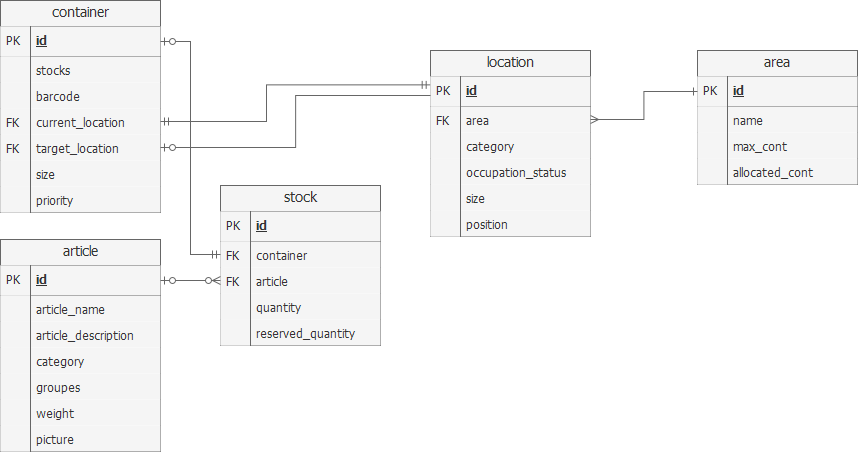
\includegraphics[width=0.6\textwidth]{DB-Schema.png}
    \centering
    \caption{Datenbankschema des AFSS}
    \label{DB-Scema}

\end{figure}

Wie in \ref{DB-Scema} ersichtlich, beinhäklt sich diese Datenbank fünf Tabellen. Diese hohe Komplexität resultiert daraus, dass diese Struktur eine 100\%ige Flexivilität in der Ablage von Bauteilen in einem überliegendem System bietet.

Die Erste Tabelle beschreibt ein einziges theoretisches Bauteil. Dieses hat einen Namen, Gewicht, Beschreibung und Kategorien zur Filterung. Unter der Spalte 'picture' wird ein Dateiname gespeichert, der zu einem Bild zeigt, dass das Produkt abbildet.
Die zweite beschreibt einen Container. Im Lagersystem entspricht dieser einer Box. Diese kann mehrere `stocks' beinhalten, sowie durch einen Barcode identifiziert werden. Weiters muss jeder Container immer eine aktuelle Position (`current\_location') besitzen, an der die Box gerade ist. Im ausgelagerten (und noch nicht eingelagerten) Zustand ist diese `location' Position 0. Das Ziel der Box wird in `target\_location' gespeichert. Stimmt die aktuelle mit der Zielposition überein, so ist die Box an ihrem Ziel angelangt. Die Kategorie `size' beschreibt die Größe eines Containers und lässt somit theoretisch zu, dass in Zukunft auch unterschiedlich große Boxen zuverlässig in die richtigen Lagerplätze eingelagert werden. `priority' wird nicht verwendet.

Container und Artikel werden im sog. 'stock' verheiratet. Dieser kann als bauteilhaufen in einer Box verstanden werden. Es können also auch mehrere 'stocks' mit dem selben Container geben, dies würde mehreren verschiedenen Bauteilen in einem einzigen Copntainer entsprechen. Auch ist es möglich mehrere Container mit den selben 'stocks' abzubilden, welches ener aufteilung von Abuteilen auf mehrere Container entspräche.

Die Positionen der Container werden in Standorte ('locations') abgebildet. Diese entsprechen den Lagerplätzen. Sie sind einer darüberliegenden 'area' zugeordnet, welche einerseits einen Lagerschrank, aber weiters auch Module wie Vereinzelungsanalgen, abbilden kann. Standorte verfüghen weiters über eine Position welche in X, Y und Z-Richtung beschreibt, wo sich ein Standort im Referenzsystem des Lagers befindet. Auch die größe des Lagerplatzes wird abgebildet, um sicherzustellen, dass auf jeden fall nur die richtige Größe an Box eingelagert wird.


\subsubsection{Docker}

    \begin{wrapfigure}{r}{0.3\textwidth} % 'r' for right, 'l' for left
        \vspace{-20px}
        
\includegraphics[width=0.3\textwidth]{docker-logo-011.png} % Replace with your image file
        \caption{Docker-Logo: \cite{docker_logo}}
    \end{wrapfigure}

    Docker ist eine Umgebung, in der Softwareprojekte isoliert werden können. Da besonders auch bei Projekten mit großem Python anteil, viele Pakete mit verschiedenen Versoinen benötigt werden, ist es sehr hilfreich diese zu bündeln. \\
    Umgesetzt wird dies mithilfe von Containern welche einen gesamten Programmteil als alleinstehende Einheit enthält. Diese werden über ein 'Dockerfile' configuriert, welches sich im selben Ordner wie die Python-Anwendung befindet. In diesem werden Parameter wie die Python-Version und die benötigten pip-Pakete sowie den Programmeinstiegspunkt angegeben. \\ 
    Ein zweier Docker Conteianer wird mit einem MySQL-Image erstellt, dort wird die Datenbank aufgesetzt. \\
    Um diese Zwei Container miteinander Kommunizieren zu lasen, ist es ntig ein sog. docker-compose.yml File zu erstellen. Dies enthält alle Informationen über verwendete container, deren Ports, sowie Speicher für Dateien (Volumes). Bei Testbetrieb wird der Datenbankcontainer aleinstehend bestrieben und mit einem anderen Port, keine Zugriffsprobleme zu generieren. In Produktion wird dann derselbe Container in den Containerverband übertragen und dort mit einem anderen Port weiterverwendet. \\
    Erstellt wird dieser Containerverband mit den Consolenbefehlt der auf das docker-compose File zugreift. 
    \begin{lstlisting}[language=bash]
        docker build docker-compose.yml\end{lstlisting}
    Dann werden auch alle Logs in der Kommandozeile ausgegeben sowie 


\subsubsection{Backend}
\subsubsection{APIs}
\subsubsection{Lageralgorithmus}
\subsubsection{Artikelsuche}
\paragraph{TF-IDF und Rust Implementierung} \hspace{0pt} \\
Der TF-IDF (Term Frequency-Inverse Document Frequency) Algorithmus, ist ein Weg um wichtige wörter aus Dokumenten zu extrahieren. Er wird verwendet um beispielsweise in Suchmaschienen, eine Suchanfrage mit Webpagecontent abzugleichen, und die am besten mit der Suchanfrage übereinsteimmenden Dokumente zu sortieren. \\
Im Fall dieser Anwendung werden die Daten aus der Artikeldatenbank als 'Dokumente'  angesehen und die Suchanfrage aus dem Suchfeld wird dafür verwendet um die am besten passenden Artikel zu finden.
\\
Durch den Relativ hohen Rechenaufwand bei dieser Suchoperation wird dieser in der Programmiersprache Rust implementert. Die Implementierung in Rust ist im vergleich zu Python schon bei relativ kleinen Datenmenge bis zu 5-mal schneller.

\subparagraph{Rust}
Rust ist eine sehr effiziente und schnelle Programmiersprache die in den späten 2000er und frühen 2010ern bei Mozilla und der Open-Source-Community entwickelt. Sie unterstützt unter anderem mehr Typensicherheit und verhindert viele Programmierfehler. 

Die Funktion dieses Algorithmus ist in drei unterteile Unterteilt.

\begin{enumerate}
    \item Term Frequenz \\
    Die Termfrequenz gibt an, wie oft ein angegebenes Wort in einem Dokument vorhanen ist. Dies wird durch die Folgende Funktion kalkuliert.
    
    \begin{lstlisting}[language=Rust]
fn term_frequency(document: &str, term: &str) -> f64 {
    // Store the lowercase document as a String to ensure it lives long enough
    let lower_document = document.to_lowercase(); 

    // Split the document into words
    let normalize_document: Vec<&str> = lower_document.split_whitespace().collect();
    // Make sure the searchterm is lowercase
    let normalize_term = term.to_lowercase();

    // Count occurrences of the term in the document
    let count = normalize_document
        .iter()
        .filter(|&&word| word == normalize_term) // Compare each word with the term
        .count();

    // Calculate the term frequency as occurrences / total number of words
    let total_words = normalize_document.len();
    if total_words == 0 {
        0.0 // Avoid division by zero if the document is empty
    } else {
        count as f64 / total_words as f64
    }
}\end{lstlisting}

    Mithilfe dieser wird eine Liste aller Wörter und der Vorkommenshäufigkeit dieser erstellt.

    \item Die zweite Komponente ist dann die Inverse Dokument Frequenz. Diese gewichtet, die Anzahl der Dokumente in dem das gesuchte Wort enthalten ist relativ zur Gesamtdokumentanzahl vorkommt. Häufig vorkommende Worte wie z.B. 'und' werden hierbei weniger gewichtet als einzigartige Wörter.

\begin{lstlisting}[language=Rust]
fn inverse_document_frequency(term: &str, all_documents: &Vec<String>) -> f64 {
    let mut num_documents_with_this_term = 0;

    // Iterate over all documents to check if they contain the term
    for doc in all_documents {
        // Normalize both term and document by converting them to lowercase
        let lower_doc = doc.to_lowercase();
        let normalized_doc: Vec<&str> = lower_doc.split_whitespace().collect();

        // Check if the term exists in the document
        if normalized_doc.contains(&term.to_lowercase().as_str()) {
            num_documents_with_this_term += 1;
        }
    }

    // Calculate IDF
    if num_documents_with_this_term > 0 {
        // Apply the IDF formula: 1 + log(total_documents / documents_with_term)
        1.0 + ((all_documents.len() as f64) / (num_documents_with_this_term as f64)).ln()
    } else {
        // If the term is not found in any document, return 1.0
        1.0
    }
}
\end{lstlisting}

    \item Nun liegt Liste davon vor, wie oft ein Wort in den Suchdaten vorkommt, als auch, wie oft ein Suchbegriff in einem bestimmten Dokument ist. \\ Als nächsten Schritt werden diese beiden Werte für jeden Suchbegriff miteinander multipliziert und ergeben somit einen Vektor der die Suchwörter in Relation zu jedem einzelnen Dokument stellt.
    \item Als letzten Schritt wird der zuvor errechnete Dokumentenvektor (der IDF jedes Suchterms in jedem Dokument) mit dem Suchvektor verglichen. Die geschieht mit der sog. Kosinus-Ähnlichkeit.
    \begin{lstlisting}[language=Rust]
fn cos_similarity(query_p: Vec<f64>, document_p: Vec<f64>) -> f64 {
    // Ensure that both vectors have the same length
    if query_p.len() != document_p.len() {
        return -1.0;
    }

    let mut dot_product = 0.0;
    let mut abs_doc_squared = 0.0;
    let mut abs_query_squared = 0.0;

    // Calculate the dot product and the magnitudes (squared)
    for i in 0..query_p.len() {
        dot_product += query_p[i] * document_p[i];
        abs_doc_squared += document_p[i].powi(2); // document_p[x] ** 2
        abs_query_squared += query_p[i].powi(2); // query_p[x] ** 2
    }

    // Calculate the magnitudes
    let abs_doc = abs_doc_squared.sqrt();
    let abs_query = abs_query_squared.sqrt();

    // Handle division by zero in case of zero vectors
    if abs_doc == 0.0 || abs_query == 0.0 {
        return 0.0;
    }

    // Return the cosine similarity
    return dot_product / (abs_doc * abs_query);
}\end{lstlisting}
    Nach der Berechnung dieser für jedes Dokument werden alle Dokumente sortiert und ausgegeben.
\end{enumerate}






